
\documentclass{article}

\usepackage[latin1]{inputenc}
\usepackage{caption}

\usepackage{tikz}
\usetikzlibrary{arrows,calc,positioning,shadows,shapes,matrix}
\usetikzlibrary{fit,chains,arrows.meta,shapes.geometric}
\usetikzlibrary{datavisualization.formats.functions}

\usepackage[american,siunitx]{circuitikz}
\usepackage{pgfplots}
\usepackage{schemabloc,calc,blox}

\usepackage{pgfplots}
%\usepgfplotslibrary{external}
%\tikzexternalize[prefix=tikz/]

\usepackage[miktex]{gnuplottex}


\begin{document}
%\pagestyle{empty}

from https://tex.stackexchange.com/questions/9386/difference-between-right-of-and-right-of-in-pgf-tikz website.

centre-to-centre placing while using \texttt{right of=} option in tikz

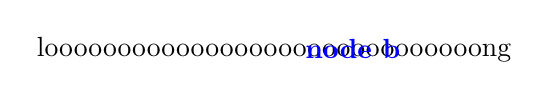
\begin{tikzpicture}
\node (a) {loooooooooooooooooooooooooooooong};
\node[right of=a,font=\bfseries,blue] (b) {node b};
\end{tikzpicture}

boundary-to-boundary placing while using \texttt{right=of} option in tikz

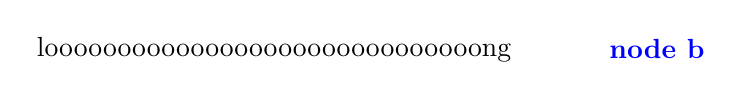
\begin{tikzpicture}
\node (a) {loooooooooooooooooooooooooooooong};
\node[right=of a,font=\bfseries,blue] (b) {node b};
\end{tikzpicture}




% ---------------------------------------------------------
\vspace{5ex}

from https://tex.stackexchange.com/questions/354401/how-to-draw-a-vector-diagram-with-tikz-datavisualization


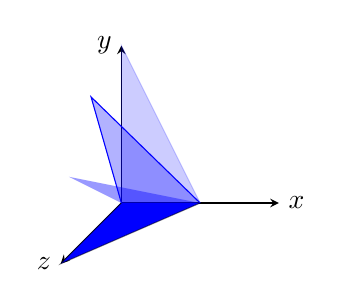
\begin{tikzpicture}[>=stealth]
\draw [->] (0,0,0) -- (2,0,0) node [at end, right] {$x$};
\draw [->] (0,0,0) -- (0,2,0) node [at end, left] {$y$};
\draw [->] (0,0,0) -- (0,0,2) node [at end, left] {$z$};

\filldraw [blue, opacity=0.2, rotate around x=0] (0,0,0) -- (0,2,0) -- (1,0,0);
\filldraw [blue,fill opacity=0.3, rotate around x=30] (0,0,0) -- (0,2,0) -- (1,0,0);
\fill [blue,fill opacity=0.4, rotate around x=60] (0,0,0) -- (0,2,0) -- (1,0,0);
\draw [fill=blue,draw opacity=0.5, rotate around x=90] (0,0,0) -- (0,2,0) -- (1,0,0);
\end{tikzpicture}



% ---------------------------------------------------------

 from https://www.overleaf.com/learn/latex/Pgfplots\_package

%\tikzexternalize
\pgfplotsset{width=10cm,compat=1.9}
\begin{tikzpicture}
\begin{axis}
\addplot[color=red]{exp(x)};
\end{axis}
\end{tikzpicture}

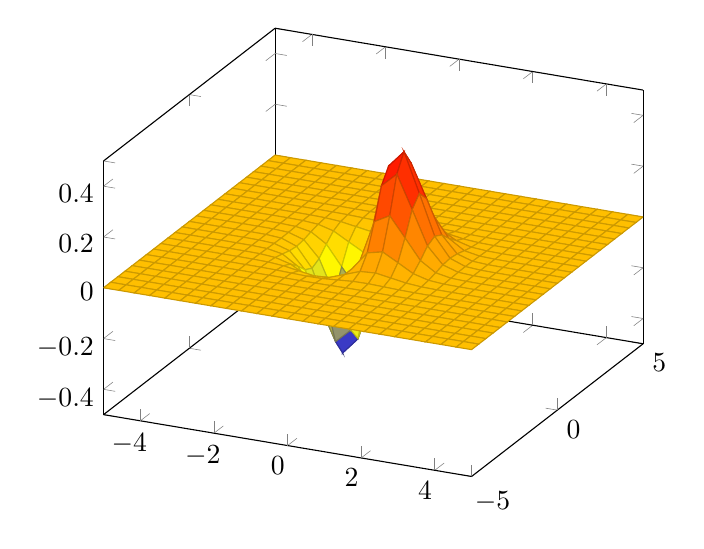
\begin{tikzpicture}
\begin{axis}
\addplot3[surf,]
{exp(-x^2-y^2)*x};
\end{axis}
\end{tikzpicture}


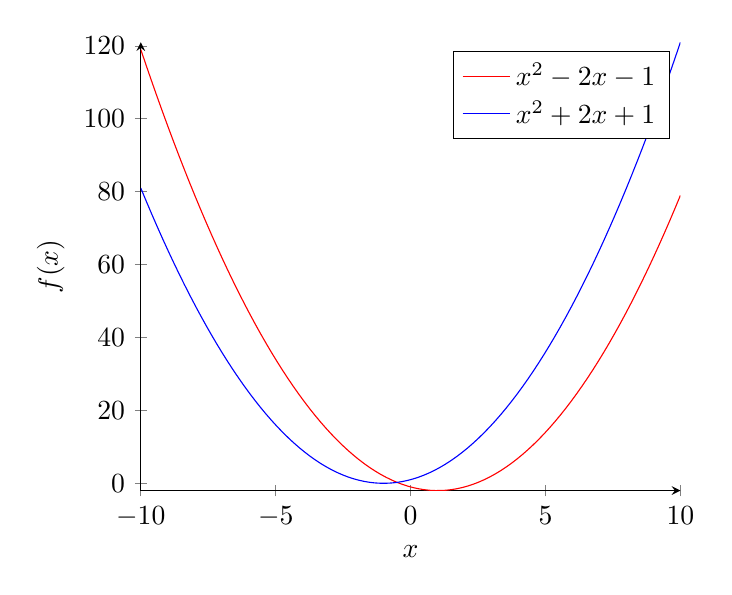
\begin{tikzpicture}
\begin{axis}[axis lines = left,xlabel = \(x\),ylabel = {\(f(x)\)},]
\addplot [domain=-10:10, samples=100, color=red,]
{x^2 - 2*x - 1};
\addlegendentry{\(x^2 - 2x - 1\)}

\addplot [domain=-10:10, samples=100, color=blue,]
{x^2 + 2*x + 1};
\addlegendentry{\(x^2 + 2x + 1\)}
\end{axis}
\end{tikzpicture}


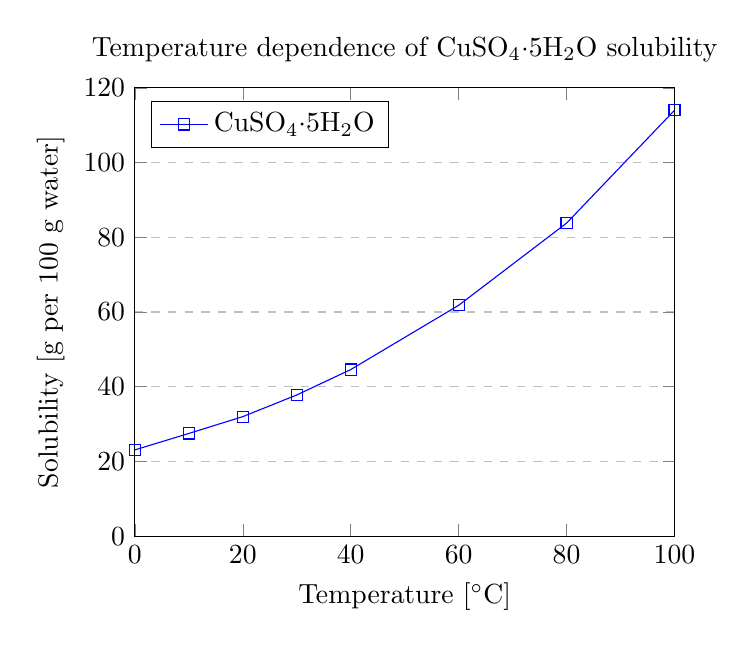
\begin{tikzpicture}
\begin{axis}[title={Temperature dependence of CuSO\(_4\cdot\)5H\(_2\)O solubility},xlabel={Temperature [$^\circ$C]}, ylabel={Solubility [g per 100 g water]}, xmin=0, xmax=100, ymin=0, ymax=120,
xtick={0,20,40,60,80,100}, ytick={0,20,40,60,80,100,120},
legend pos=north west, ymajorgrids=true, grid style=dashed,]
\addplot[color=blue, mark=square,]
coordinates {	(0,23.1)(10,27.5)(20,32)(30,37.8)(40,44.6)(60,61.8)(80,83.8)(100,114)};
\legend{CuSO\(_4\cdot\)5H\(_2\)O}
\end{axis}
\end{tikzpicture}


\begin{tikzpicture}
\begin{axis}[enlargelimits=false,]
	\addplot+[only marks,scatter,mark=halfcircle*,mark size=2.9pt]
	table[meta=ma]{scattered_example.dat};
\end{axis}
\end{tikzpicture}


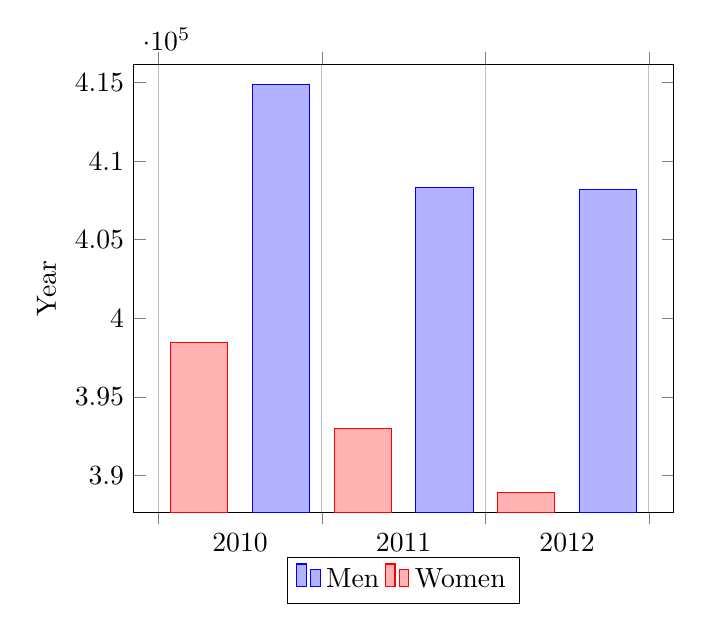
\begin{tikzpicture}
\begin{axis}[x tick label style={/pgf/number format/1000 sep=}, ylabel=Year, enlargelimits=0.05, legend style={at={(0.5,-0.1)}, anchor=north, legend columns=-1}, ybar interval=0.7, ]
\addplot coordinates {(2012,408184) (2011,408348) (2010,414870) (2009,412156)};
\addplot coordinates {(2012,388950) (2011,393007) (2010,398449) (2009,395972)};
\legend{Men,Women}
\end{axis}
\end{tikzpicture}


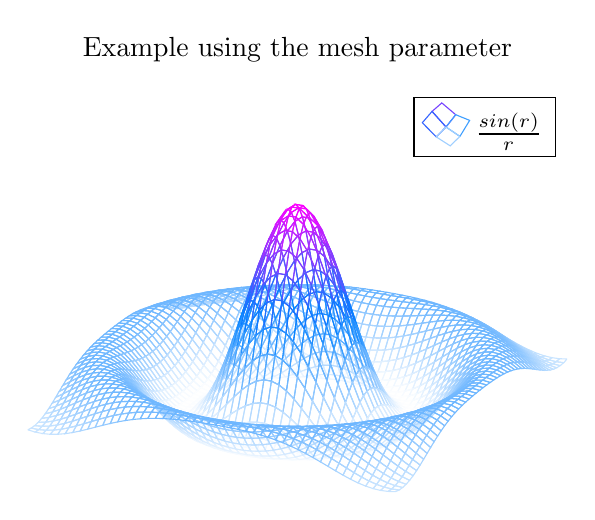
\begin{tikzpicture}
\begin{axis}[title=Example using the mesh parameter,hide axis,colormap/cool,]
\addplot3[mesh, samples=50, domain=-8:8,]
{sin(deg(sqrt(x^2+y^2)))/sqrt(x^2+y^2)};
\addlegendentry{\(\frac{sin(r)}{r}\)}
\end{axis}
\end{tikzpicture}


\begin{tikzpicture}
\begin{axis}[title={Contour plot, view from top}, view={0}{90} ]
\addplot3[contour gnuplot={levels={0.8, 0.4, 0.2, -0.2}} ]
{sin(deg(sqrt(x^2+y^2)))/sqrt(x^2+y^2)};
\end{axis}
\end{tikzpicture}


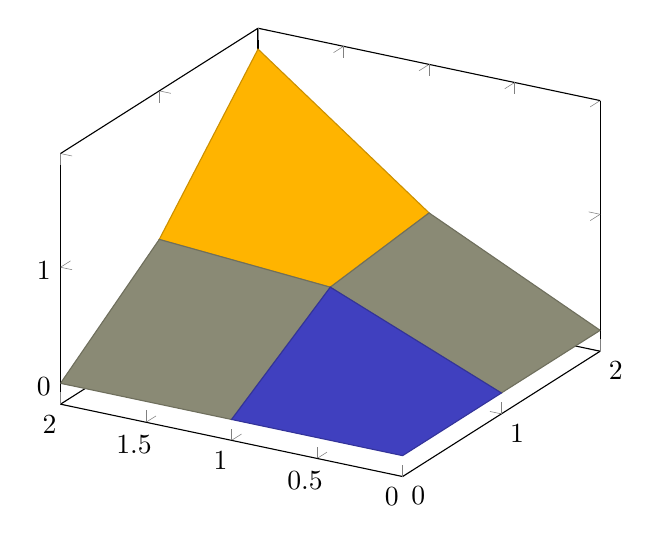
\begin{tikzpicture}
\begin{axis}[view={-60}{30},]
\addplot3[surf,] 
coordinates {(0,0,0) (0,1,0) (0,2,0)
	
	(1,0,0) (1,1,0.6) (1,2,0.7)
	
	(2,0,0) (2,1,0.7)(2,2,1.8)};
\end{axis}
\end{tikzpicture}


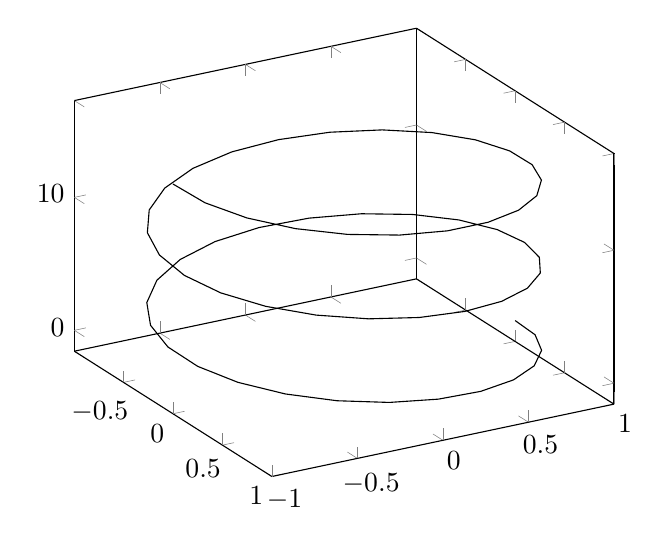
\begin{tikzpicture}
\begin{axis}[view={60}{30},]
\addplot3[domain=0:5*pi,samples = 60,samples y=0,]
({sin(deg(x))},{cos(deg(x))},{x});
\end{axis}
\end{tikzpicture}



% ================================================

from https://stackoverflow.com/questions/36386656/how-to-plot-in-latex-with-gnuplot


\begin{figure}[h]  \centering
\begin{gnuplot}[terminal=epslatex]
	set terminal epslatex color size 14.5cm, 6cm
	set key top left
	set xlabel '$ x [1] $'
	set ylabel '$ y [1] $'
	f1(x)=sin(x**2)
	plot f1(x) title '$ y_1 = \sin(x^2) $'
\end{gnuplot}
\caption{Plot}
\end{figure}



% ================================================

from https://tex.stackexchange.com/questions/136288/pgfplots-how-to-fill-area-under-a-curve-in-a-3d-plot-similar-to-closedcycle-in

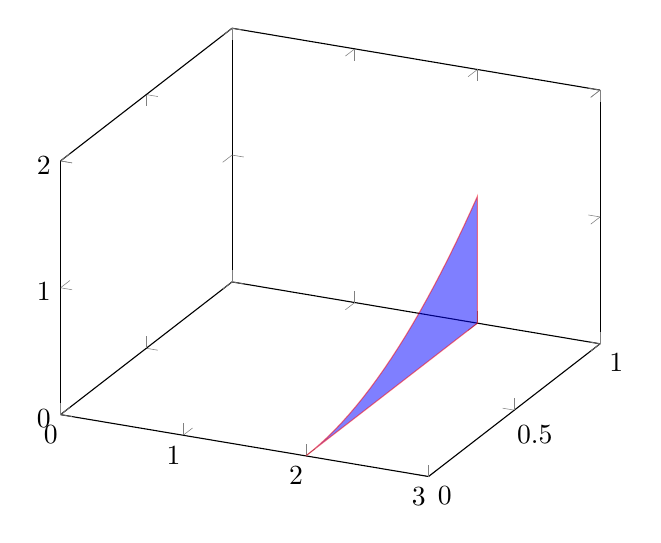
\begin{tikzpicture}
\begin{axis}[xmin=0,xmax=3,zmin=0,zmax=2]
\addplot3[red,domain=0:1,fill=blue,opacity=0.5,samples y=0] (2,x,x^2) -- (axis cs:2,1,0) -- (axis cs:2,0,0);
\end{axis}
\end{tikzpicture}



% ================================================






\end{document} 